%!TEX root = ../report.tex

% 
% Architecture
% 

\section{Solution's Architecture Proposal}

Considering this project's problem and the objectives presented in problem contextualization section, We want to develop a process framework for project and maintenance management to be applied to an Information Systems administration. We provided, in Related Work section, a state of the art in several frameworks for IT governance and management, as well as international standards, building a knowledge base to start planning and designing the processes.\par
Taking in account the complexity of some frameworks presented, like COBIT, and also the problem's scope and the solution time-frame, we need to conduct an analysis of the knowledge we will use from each framework or standard. We will use ISO/IEC 12207, presented in section 5.1, to define which types of processes we will consider for this project, defining next the frameworks and standards we will consider as reference for each type of processes. As long as processes need supporting artifacts and a responsibility structure, this references also support this needs, presenting some suggestions of how responsibilities are addressed for each process and what artifacts are needed for a correct implementation.\par
Since we are also looking for a logical application architecture, we will provide a deeper analysis on the solutions present in section 6, narrowing down the available solutions to provide the features more important for this project, in order to reach an logical application architecture that is able to fully support our process framework.\par
As long as this project is aligned with a real-case scenario for an organization, we will take design decisions considering the stakeholders for this project, specially when dealing with the choice of the type of processes to consider and the solutions chosen for integrating the logical application architecture. This organization will also provide us ways to demonstrate our solution's suitability, allowing us to achieve the demonstration and evaluation step of the DSRM process applied for this project.\par



\subsection{Process Framework}

To start designing our processes, we need first to define what processes we will consider to be in the scope of this project. For this, and taking as reference ISO/IEC 12207, detailed in section 5.1, that standardizes the processes for the whole life cycle of software, we will present the areas we will address and the reasons why we do not do it for the others.\par
The two main areas to consider are governance and management processes. Considering the extensibility and complexity of both, we could not focus on the two, giving the time-frame available. Being so, we decided, accordingly with the stakeholders, to not detail governance processes. Areas focused on organization strategy or project portfolio will not be addressed for this project. Instead, we will consider that this subjects are already clearly defined by the organization, being our responsibility designing processes that comply with them. 
Despite this, there are governance processes that will have direct influence on the subjects covered by this thesis, namely risk, budget and quality management. These subjects will be addressed by this project considering a more operational approach. We will consider that organization strategy for this areas is already defined, being our mission design processes that implement and ensure this strategy in practice.\par


\subsubsection{Processes definition}


The areas of interest were chosen based on stakeholders' needs for this project. As long as it is aligned with a real-case organization, we had to proceed to interviews with stakeholders as a way to define the problem, namely the areas of interest we need to cover. This areas were chosen in agreement with the two parties involved in this project, bu it can be changed during project execution.\par
Our idea with this project is to provide a more general process framework for project and maintenance management, but that would be applicable to this organization particular scenario. Based on this, the processes we will consider are aligned with this objective, being, in our shared opinion, the most important to consider in this scenario. Also, more areas can be covered in the future, if we consider it is a added value for this framework.  
In figure 32 we can observe the areas of interest for this project highlighted from the ISO/IEC 12207 international standard. This standard was considered because we needed a starting point to define the processes scope for this project. Groups of processes directly related to governance are not considered for this project, as well as the Agreement processes and Organizational Project-Enabling processes.\par
Technical Processes and Software Implementation processes are also not considered in the scope, because we will assume that project's implementation is outsourced, being responsibility of a third-party. In light of this, processes presented in Technical and Software Implementation processes groups are not relevant for the organization, although they are fundamental for the third-party that will implement the project. Despite this assumption, the organization itself has a complete process for project management, that is different from the third-party project. Aspects like project calendar, deliveries and control are done by the two entities by different perspectives, being us responsible for the organization project management.\par
For this thesis, we will consider the Project processes and the Software Support processes, both directly related to project and maintenance management. In addition to the processes in Project processes group, we will also consider Capacity Management, Issues Management,Financial Management and Document Management as processes belonging to this group.\par
Regarding Software Support Processes, we will consider Software Documentation Management, Software Configuration Management and Software Validation processes.\par
Software Reuse Processes group will not be considered for this project because it is not considered as a theme of interest for it, being also not related with the objectives we purpose. 

\begin{figure}[h!]
\centering
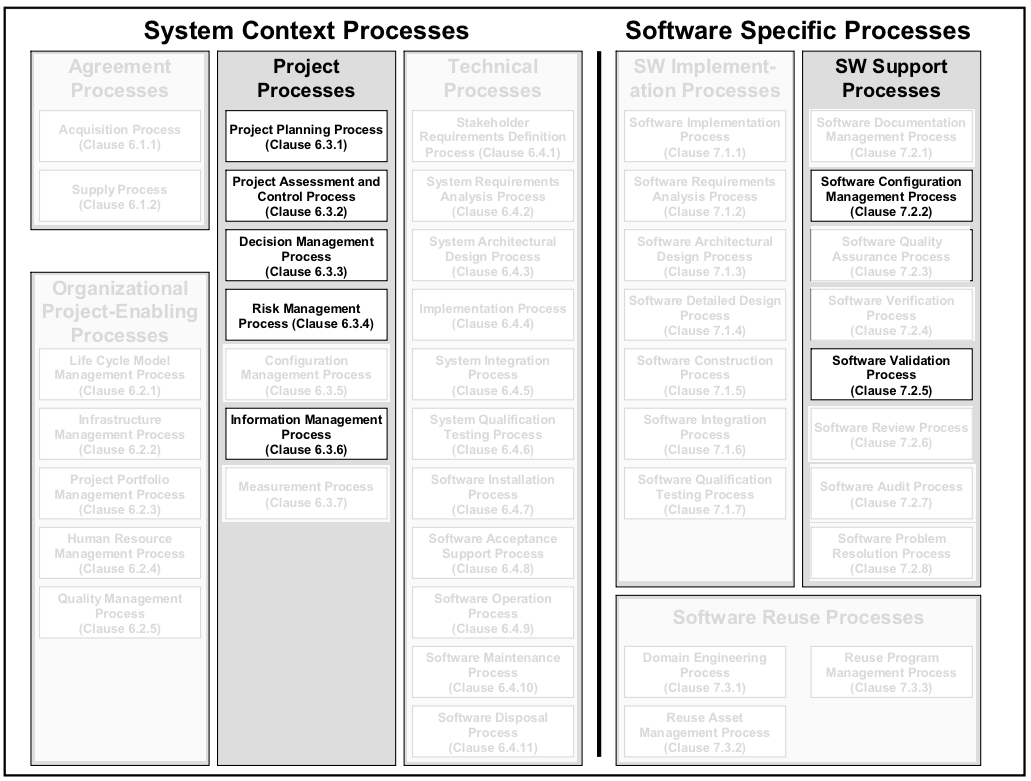
\includegraphics[width=0.8\textwidth]{img/ISO12207ProcessesImplemented.png}
\caption{Processes areas considered for this project. Adapted from \cite{ISO12207}.}
\end{figure}

Capacity Management, issues Management, Financial Management and Document Management are process areas that are not clearly addressed by ISO/IEC 12207, but are processes necessary to consider based on stakeholders' needs.\par
Capacity Management, as stated in \cite{itilSD}, ``ensure that cost-justifiable IT capacity in all areas of IT always exists and is matched to the current and future agreed needs of the business, in a timely manner.''. It is point were all performance and capacity subjects are dealt, considering resources and services itself. Capacity management is focused on two operations: balancing costs against resources needed and balancing supply against demand.\par
Capacity Management is divided in three main areas: Business Capacity Management (business needs and plans' translation into requirements for service and IT infrastructure), Service Capacity Management (management, control and prediction of performance and capacity of IT services operation) and Component Capacity Management (management, control and prediction of the performance, utilization and capacity of individual IT technology components).\par
Issues Management is the process of identifying and resolving issues, as staff, supplier, technical or material problems. Many times confused with risks, issues have a more unpredictable profile. They can arise from project processes with no warning or no expectation at all. Most organizations find difficult to manage issues from an effectively manner and many times it a process that is not implemented across the complete organization, making more difficult its resolution.\par
As stated in \cite{itilSS}, ``Financial Management provides the business and IT with the quantification, in financial terms, of the value of IT Services, the value of the assets underlying the provisioning of those services, and the qualification of operational forecasting''. As the main areas for IT Financial Management we have Budgeting (Expenditures planning and controlling), IT accounting (Cost analysis on IT services providing) and Charging (Costs assignment to IT services provided). Financial Management is a complex area and we need a more deeper analysis on its importance for our framework, in order to only provide the needed financial activities.\par
Documentation Management corresponds to an area that deals with all documentation concerns on an organization, from technical to project management documentation. This area groups processes for plan, production, tracking and communication of documents produced by the organization in project and maintenance contexts. This processes are also related to the supporting artifacts we want to develop and need to be taken in account to achieve success for the whole processes.\par
In table 2 is presented a table with the processes group we will consider for this project and a description of some activities each process intents to implement.

\begin{table}[h!]
\centering
\resizebox{\textwidth}{!}{%
\begin{tabular}{|l|c|c|c|c|c|c|c|c|c|c|c|c|c|}
\hline
\multicolumn{1}{|c|}{} & \multicolumn{4}{c|}{\textbf{COBIT 5 Domains}} & \multicolumn{5}{c|}{\textbf{ITIL V3 Volumes}} &  &  &  &  \\ \cline{2-10}
\multicolumn{1}{|c|}{\multirow{-2}{*}{\textbf{Processes}}} & \textbf{APO} & \textbf{BAI} & \textbf{DSS} & \textbf{MEA} & \textbf{SS} & \textbf{SD} & \textbf{SO} & \textbf{ST} & \textbf{CSI} & \multirow{-2}{*}{\textbf{PMBOK}} & \multirow{-2}{*}{\textbf{\begin{tabular}[c]{@{}c@{}}ISO/IEC\\ 20000\end{tabular}}} & \multirow{-2}{*}{\textbf{\begin{tabular}[c]{@{}c@{}}ISO/IEC \\ 27000\end{tabular}}} & \multirow{-2}{*}{\textbf{\begin{tabular}[c]{@{}c@{}}ISO\\ 31000\end{tabular}}} \\ \hline
\textbf{Project Planning} & \cellcolor[HTML]{5A9D58}\checkmark & \cellcolor[HTML]{5A9D58}\checkmark &  &  &  &  &  &  &  & \cellcolor[HTML]{FD6864}\checkmark & \cellcolor[HTML]{329A9D}\checkmark &  &  \\ \hline
\textbf{Project Assessment and Control} & \cellcolor[HTML]{5A9D58}{\color[HTML]{000000} \checkmark} & \cellcolor[HTML]{5A9D58}{\color[HTML]{000000} \checkmark} & \cellcolor[HTML]{5A9D58}{\color[HTML]{000000} \checkmark} & \cellcolor[HTML]{5A9D58}{\color[HTML]{000000} \checkmark} &  &  &  &  &  & \cellcolor[HTML]{FD6864}\checkmark & \cellcolor[HTML]{329A9D}\checkmark &  &  \\ \hline
\textbf{Decision Management} & \cellcolor[HTML]{5A9D58}{\color[HTML]{000000} \checkmark} & \cellcolor[HTML]{5A9D58}{\color[HTML]{000000} \checkmark} & \cellcolor[HTML]{5A9D58}{\color[HTML]{000000} \checkmark} & \cellcolor[HTML]{5A9D58}{\color[HTML]{000000} \checkmark} & \cellcolor[HTML]{FFCC67}\checkmark &  &  &  &  & \cellcolor[HTML]{FD6864}\checkmark & \cellcolor[HTML]{329A9D}\checkmark &  &  \\ \hline
\textbf{Risk Management} & \cellcolor[HTML]{5A9D58}\checkmark &  &  &  &  & \cellcolor[HTML]{FFCC67}\checkmark &  &  &  & \cellcolor[HTML]{FD6864}\checkmark &  & \cellcolor[HTML]{329A9D}\checkmark & \cellcolor[HTML]{329A9D}\checkmark \\ \hline
\textbf{Capacity Management} & \cellcolor[HTML]{5A9D58}\checkmark & \cellcolor[HTML]{5A9D58}\checkmark &  &  &  & \cellcolor[HTML]{FFCC67}\checkmark &  &  &  &  &  &  &  \\ \hline
\textbf{Issues Management} &  &  & \cellcolor[HTML]{5A9D58}\checkmark &  &  &  & \cellcolor[HTML]{FFCC67}\checkmark &  &  &  &  &  &  \\ \hline
\textbf{Financial Management} & \cellcolor[HTML]{5A9D58}\checkmark &  &  &  & \cellcolor[HTML]{FFCC67}\checkmark &  &  &  &  &  &  &  &  \\ \hline
\textbf{Documentation Management} & \cellcolor[HTML]{5A9D58}\checkmark & \cellcolor[HTML]{5A9D58}\checkmark &  &  &  &  &  &  &  & \cellcolor[HTML]{FD6864}\checkmark &  & \cellcolor[HTML]{329A9D}\checkmark &  \\ \hline
\textbf{Software Configuration Management} &  & \cellcolor[HTML]{5A9D58}\checkmark &  &  &  &  &  & \cellcolor[HTML]{FFCC67}\checkmark &  &  &  &  &  \\ \hline
\textbf{Software Validation} & \cellcolor[HTML]{5A9D58}\checkmark &  &  &  &  &  &  & \cellcolor[HTML]{FFCC67}\checkmark &  & \cellcolor[HTML]{FD6864}\checkmark &  &  &  \\ \hline
\end{tabular}
}
\vspace{2mm}
\caption{Processes areas and main activities.}
\label{my-label}
\end{table}


\subsubsection{Processes Mapping to frameworks}

In this section we will present how each one of the processes in the scope for this project are addressed and mapped into the frameworks and standards presented in section 4 and 5. This will provide us an initial guidance on how we should approach the problem, based on already stated knowledge by professionals in the area. Our objective is to use only the important aspects for this project, reducing the complexity of implementing a complete framework for the organization. Consider this, we need to map the processes in the scope for this project to, during processes design, discover what objectives are already covered by the frameworks and which ones need more original work.\par
In table 3 we present the mapping between each processes group in the scope for this project with the framework or standard that covers some aspects for it:\par

\begin{table}[h!]
\centering
\resizebox{0.9\textwidth}{!}{%
\begin{tabular}{|c|l|}
\hline
\textbf{Processes} & \multicolumn{1}{c|}{\textbf{Description}} \\ \hline
\textbf{Project Planning} & \begin{tabular}[c]{@{}l@{}}Scope and goals definition;\\ Requirements establishment;\\ Activities and deliverables identification;\\ Schedule definition;\\ Resources identification;\\ Responsibilities assignment;\\ Quality, Risk and Cost Analysis;\end{tabular} \\ \hline
\textbf{Project Assessment and Control} & \begin{tabular}[c]{@{}l@{}}Project monitoring;\\ Project control;\\ Project assessment;\end{tabular} \\ \hline
\textbf{Decision Management} & \begin{tabular}[c]{@{}l@{}}Decision-Making strategy definition;\\ Alternative Courses of action definition;\\ Course of action identification;\\ Decision analysis;\\ Decision tracking;\end{tabular} \\ \hline
\textbf{Risk Management} & \begin{tabular}[c]{@{}l@{}}Risk Management planning;\\ Risk Profile Management;\\ Risk Analysis;\\ Risk Treatment;\\ Risk Monitoring;\\ Risk Management process evaluation;\end{tabular} \\ \hline
\textbf{Capacity Management} & \begin{tabular}[c]{@{}l@{}}Capacity Plan definition;\\ Performance Monitoring;\\ Performance Analysis;\\ Performance tuning;\end{tabular} \\ \hline
\textbf{Issues Management} & \begin{tabular}[c]{@{}l@{}}Issue Identification;\\ Issue Prioritization;\\ Issue Resolution;\\ Issue Communication;\end{tabular} \\ \hline
\textbf{Financial Management} & \begin{tabular}[c]{@{}l@{}}Budgeting definition;\\ IT Accounting planning;\\ Charging planning;\\ Financial control;\\ Financial communication;\end{tabular} \\ \hline
\textbf{Documentation Management} & \begin{tabular}[c]{@{}l@{}}Documentation definition;\\ Documentation production;\\ Documentation validation;\\ Documentation communication;\\ Documentation tracking;\end{tabular} \\ \hline
\textbf{Software Configuration Management} & \begin{tabular}[c]{@{}l@{}}Software configuration management plan developing;\\ Configuration Identification;\\ Configuration Control;\\ Configuration Status Accounting;\\ Configuration Evaluation;\end{tabular} \\ \hline
\textbf{Software Validation} & \begin{tabular}[c]{@{}l@{}}Validation plan definition;\\ Test requirements, test cases and test specifications preparation;\\ Tests Execution;\\ Software validation against the requirements execution;\end{tabular} \\ \hline
\end{tabular}
}
\vspace{2mm}
\caption{Processes Mapping to frameworks and standards.}
\label{my-label}
\end{table}

\subsubsection{Processes Supporting artifacts}

Considering the framework we want to develop, we need some artifacts to support this processes, namely communication and decisions artifacts that will allow us to support the inputs and outputs for activities in each process. For this, we will provide, in conjunction with the processes framework, all artifacts needed to support it, clearly defining its purpose, content and participants.\par
This artifacts will be defined during the designing of the process framework. The frameworks and standards previously presented define some of them,  being our work to address new artifacts that are not covered by any of the frameworks and standards.\par

\subsubsection{Responsibility Structure}

The developed framework needs to have an inherent responsibility structure, defining the processes' participants accounted for decisions and activities. This structure is particularly important when considering we are dealing with a real-case organization, that has already an organizational structure defined and for the one we are designing our processes.\par
For designing this responsibility structure we will consider the work already done in responsibility assignment for the frameworks and standards previously presented. COBIT and ITIL define clearly the responsibility structure for its processes. Despite that, we need also to have some original work on this subject, considering we are not implementing directly any of those frameworks. This work will be accomplished during the processes' design and taking in account the common responsibility structures on IT organizations.\par 

\subsection{Logical Application Architecture}

A proposal for a logical application architecture is one of the objectives of this project, being important to support the processes framework. To achieve this, we evaluated a set of PPM and ITSM Solutions available in the market with the objective of achieving a proposal of applications that can be a part of this architecture.\par
For evaluation purposes, we used Gartner and Forrester research, presented in section 6, that allow us to independently evaluate how these tools stand a position in the PPM and ITSM Market and also what are the solutions more complete in terms of features and capacities.\par
In this section we will present the solutions we consider the best for our objectives, being part of a proposal for the project's stakeholders. After deciding what solution we will consider for this project, we need to design a logical application architecture, where we will present how the processes are supported by our applications and how it is integrated.\par

\subsubsection{PPM Tools}

For PPM solutions, that we evaluate in section 6.3, we used the Magic Quadrant , the MarketScope and the Forrester Wave methodologies for evaluation.\par
In Magic Quadrant results, that presents how well solutions' providers conform with market needs, we will just consider the leaders quadrant, composed by Planview, Compuware, CA, HP, Oracle and Microsoft. Planview and CA are the suppliers with the best results but are closely followed by the rest. A deeper analysis on strengths and cautions presented by Gartner for each one of this solutions is presented in \cite{magicQuadrantPPM}.\par
In MarketScope results, that presents how well solutions deal on emerging markets with changing requirements, we will only consider the solutions with strong positive and positive ratings. This method is particular important in this area, because PPM solutions are facing market changes, looking more for Cloud based solutions in the future. As well as on magic Quadrant, Planview and CA Techncologies present the best results with strong positive ratings. The other solutions we are considering obtained positive rating.\par
For the Forrester Wave results, that evaluates providers by criteria and respective weightings, we will consider the two models explained in section 6.3, the above-the-line and below-the-line. For the first one, the leaders quadrant is composed by Planview, CA Technologies, HP and Daptiv. All presents good results but is CA Technologies who is the most complete provider, in terms of current offering, strategy and market presence. Other providers present better results in some of this criteria but are substantially worse in others. For the below-the-line evaluation, we have CA Technologies and Planview very close to each other and HP with an excellent result in strategy criteria. Microsoft, Rally and Daptiv are also part of the leaders, but with results slightly worse.\par
In table 3 we can observe the PPM Tools Evaluation results. In green we have the solutions we consider the best for this project taking in account the evaluation results. We also present the alternatives in orange. CA Technologies with CA Clarity PPM and Planview with Planview Enterprise are the solutions we will purpose for the PPM Tool to consider for this project.


\begin{table}[h!]
\centering
\resizebox{\textwidth}{!}{%
\begin{tabular}{|c|c|l|c|c|c|l|}
\hline
 & \multicolumn{2}{c|}{} &  & \multicolumn{3}{c|}{\textbf{Forrester Wave}} \\ \cline{5-7} 
\multirow{-2}{*}{\textbf{Solutions Providers}} & \multicolumn{2}{c|}{\multirow{-2}{*}{\textbf{\begin{tabular}[c]{@{}c@{}}Gartner\\ Magic\\ Quadrant\end{tabular}}}} & \multirow{-2}{*}{\textbf{Marketscope}} & \multicolumn{1}{l|}{\textbf{Above-The-Line}} & \multicolumn{2}{l|}{\textbf{Below-The-Line}} \\ \hline
\rowcolor[HTML]{5A9D58} 
\textbf{CA Technologies} & \multicolumn{2}{c|}{\cellcolor[HTML]{5A9D58}Leader} & Strong Positive & Leader & \multicolumn{2}{c|}{\cellcolor[HTML]{5A9D58}Leader} \\ \hline
\rowcolor[HTML]{5A9D58} 
\textbf{Planview} & \multicolumn{2}{c|}{\cellcolor[HTML]{5A9D58}Leader} & Strong Positive & Leader & \multicolumn{2}{c|}{\cellcolor[HTML]{5A9D58}Leader} \\ \hline
\rowcolor[HTML]{FFCB2F} 
\textbf{HP} & \multicolumn{2}{c|}{\cellcolor[HTML]{FFCB2F}Leader} & Positive & Leader & \multicolumn{2}{c|}{\cellcolor[HTML]{FFCB2F}Leader} \\ \hline
\rowcolor[HTML]{FFCB2F} 
\textbf{Microsoft} & \multicolumn{2}{c|}{\cellcolor[HTML]{FFCB2F}Leader} & Positive & Strong Performer & \multicolumn{2}{c|}{\cellcolor[HTML]{FFCB2F}Leader} \\ \hline
\textbf{Oracle} & \multicolumn{2}{c|}{Leader} & Positive & - & \multicolumn{2}{c|}{-} \\ \hline
\textbf{Compuware} & \multicolumn{2}{c|}{Leader} & Positive & - & \multicolumn{2}{c|}{-} \\ \hline
\textbf{Rally} & \multicolumn{2}{c|}{-} & - & Strong Performer & \multicolumn{2}{c|}{Leader} \\ \hline
\textbf{Daptiv} & \multicolumn{2}{c|}{-} & - & Leader & \multicolumn{2}{c|}{Leader} \\ \hline
\end{tabular}
}
\vspace{2mm}
\caption{PPM Tools evaluation results.}
\label{my-label}
\end{table}

\subsubsection{ITSM Tools}

For ITSM solutions, that we evaluate in section 6.4, we used the Magic Quadrant , the Critical Capabilities and the Forrester Wave methodologies for evaluation.\par
In Magic Quadrant results, that presents how well solutions' providers conform with market needs, we will just consider the leaders and challengers quadrants, composed by ServiceNow and BMC Software for the leaders and Cherwell and CA Technologies for challengers. ServiceNow is the best provider in terms of ability to execute with some advantage to concurrency but really close of BMC Software in terms of completeness of vision. Cherwell Software and CA Technologies present a considering lower result for completeness of vision considering the leaders quadrant. A deeper analysis on strengths and cautions presented by Gartner for each one of this solutions is presented in \cite{magicQuadrantITSM}.\par
In Critical Capabilities results, we will only consider the High-Maturity, Digital Workplace and Total ITSM Use Cases. We will also only consider the solutions provided by the suppliers in the leaders and challengers quadrants presented by Gartner. In all the use cases considered, BMC Remedy ITSM Suite and ServiceNow IT Service Automation suite have the higher scores, being followed by some distance by CA Service Management and Cherwell Software Service Management.\par
For the Forrester Wave results, we have Cherwell Software and Service Now as the leaders, very close to each other and with a very good result in terms of market presence. BMC Software and CA Technologies are considered Strong Performers, but at some distance of the other two. Forrester establishes big differences between the two leaders providers and the two strong contenders in terms of the three criteria considered.\par
In table 4 we can observe the ITSM Tools Evaluation results. In green we have the solution we consider the best for this project taking in account the evaluation results. ServiceNow with ServiceNow IT Service Automation is the solution we will purpose for the ITSM Tool to consider for this project. We also present other alternatives in orange. It should be taken special attention to CA Technologies tool as alternative solution if we consider the CA Technologies PPM tool due to easier integration between the PPM and ITSM tools.


\begin{table}[h]
\centering
\resizebox{\textwidth}{!}{%
\begin{tabular}{|c|c|c|c|c|c|}
\hline
 &  & \multicolumn{3}{c|}{\textbf{Gartner Critical Capabilities}} &  \\ \cline{3-5}
\multirow{-2}{*}{\textbf{\begin{tabular}[c]{@{}c@{}}Solutions\\ Providers\end{tabular}}} & \multirow{-2}{*}{\textbf{\begin{tabular}[c]{@{}c@{}}Gartner\\ Magic \\ Quadrant\end{tabular}}} & \textbf{\begin{tabular}[c]{@{}c@{}}High\\ Maturity\\ UC\end{tabular}} & \textbf{\begin{tabular}[c]{@{}c@{}}Digital \\ Workplace \\ UC\end{tabular}} & \textbf{\begin{tabular}[c]{@{}c@{}}Total\\  ITSM\\ Use Case\end{tabular}} & \multirow{-2}{*}{\textbf{\begin{tabular}[c]{@{}c@{}}Forrester \\ Wave\end{tabular}}} \\ \hline
\rowcolor[HTML]{5A9D58} 
\textbf{ServiceNow} & Leaders & 3,68 & 3,49 & 3,56 & Leader \\ \hline
\rowcolor[HTML]{FFCC67} 
\textbf{Cherwell Software} & Challengers & 3,15 & 3,12 & 3,22 & Leader \\ \hline
\rowcolor[HTML]{FFCC67} 
\textbf{BMC Software} & Leaders & 3,74 & 3,49 & 3,52 & Strong Performers \\ \hline
\rowcolor[HTML]{FFCC67} 
\textbf{CA Technologies} & Challengers & 3,39 & 3,31 & 3,22 & Strong Performers \\ \hline
\end{tabular}
}
\vspace{2mm}
\caption{ITSM Tools evaluation results.}
\label{my-label}
\end{table}

\subsection{Demonstration Proposal}

For demonstrating our solution we will apply our process framework and logical application architecture to a real-case organization, from the utilities sector of business (Energy). This organization is composed by a unique administration for applications (software) area. This administration will receive two types of requests: project execution and evolving maintenance requests. All the assumptions were made available from the stakeholder for this project, using an interview approach.\par
Considering the stakeholders for this demonstration project, we have two types: Internal and External. Considering internal stakeholders, we have the Business area, composed by the organization administration (sponsor), the financial department and logistic department and the Technology area, composed by the Information Systems department (Project execution and Maintenance project managers and leaders). Considering the external stakeholders, we have the third-parties responsible for project implementation, suppliers, consumers and regulatory entities.\par
Project Execution department will outsource project implementation to a third-party but internally will maintain processes for project management, independent from the third-party. it corresponds to the project internal administration considering the third-party activities. Evolving maintenance requests are filtered by a Help-Desk service, Wherefore only the Major Changes requests arrive to the evolving maintenance department.\par
A project only enters in production phase after approval from the maintenance department. When in production phase, project belongs to the maintenance department. Maintenance department can, accordingly with a strategical plan defined, outsource the maintenance implementation, being only responsible for its management.\par
This demonstration proposal is a specialization application of our process framework but was considered during its planning, reason why some processes were not considered to make part of the framework, because they would introduce too much complexity considering the application purposes.\par



